%% bare_conf.tex
%% V1.4b
%% 2015/08/26
%% by Michael Shell
%% See:
%% http://www.michaelshell.org/
%% for current contact information.
%%
%% This is a skeleton file demonstrating the use of IEEEtran.cls
%% (requires IEEEtran.cls version 1.8b or later) with an IEEE
%% conference paper.
%%
%% Support sites:
%% http://www.michaelshell.org/tex/ieeetran/
%% http://www.ctan.org/pkg/ieeetran
%% and
%% http://www.ieee.org/

%%*************************************************************************
%% Legal Notice:
%% This code is offered as-is without any warranty either expressed or
%% implied; without even the implied warranty of MERCHANTABILITY or
%% FITNESS FOR A PARTICULAR PURPOSE! 
%% User assumes all risk.
%% In no event shall the IEEE or any contributor to this code be liable for
%% any damages or losses, including, but not limited to, incidental,
%% consequential, or any other damages, resulting from the use or misuse
%% of any information contained here.
%%
%% All comments are the opinions of their respective authors and are not
%% necessarily endorsed by the IEEE.
%%
%% This work is distributed under the LaTeX Project Public License (LPPL)
%% ( http://www.latex-project.org/ ) version 1.3, and may be freely used,
%% distributed and modified. A copy of the LPPL, version 1.3, is included
%% in the base LaTeX documentation of all distributions of LaTeX released
%% 2003/12/01 or later.
%% Retain all contribution notices and credits.
%% ** Modified files should be clearly indicated as such, including  **
%% ** renaming them and changing author support contact information. **
%%*************************************************************************


% *** Authors should verify (and, if needed, correct) their LaTeX system  ***
% *** with the testflow diagnostic prior to trusting their LaTeX platform ***
% *** with production work. The IEEE's font choices and paper sizes can   ***
% *** trigger bugs that do not appear when using other class files.       ***                          
% The testflow support page is at:
% http://www.michaelshell.org/tex/testflow/

\documentclass[conference]{IEEEtran}
% Some Computer Society conferences also require the compsoc mode option,
% but others use the standard conference format.
%
% If IEEEtran.cls has not been installed into the LaTeX system files,
% manually specify the path to it like:
% \documentclass[conference]{../sty/IEEEtran}

\usepackage[usenames,dvipsnames]{color}
\newcommand{\todo}[1]
  {{\scriptsize \textbf{\color{red} {#1}}}}



% Some very useful LaTeX packages include:
% (uncomment the ones you want to load)


% *** MISC UTILITY PACKAGES ***
%
%\usepackage{ifpdf}
% Heiko Oberdiek's ifpdf.sty is very useful if you need conditional
% compilation based on whether the output is pdf or dvi.
% usage:
% \ifpdf
%   % pdf code
% \else
%   % dvi code
% \fi
% The latest version of ifpdf.sty can be obtained from:
% http://www.ctan.org/pkg/ifpdf
% Also, note that IEEEtran.cls V1.7 and later provides a builtin
% \ifCLASSINFOpdf conditional that works the same way.
% When switching from latex to pdflatex and vice-versa, the compiler may
% have to be run twice to clear warning/error messages.






% *** CITATION PACKAGES ***
%
\usepackage{cite}
% cite.sty was written by Donald Arseneau
% V1.6 and later of IEEEtran pre-defines the format of the cite.sty package
% \cite{} output to follow that of the IEEE. Loading the cite package will
% result in citation numbers being automatically sorted and properly
% "compressed/ranged". e.g., [1], [9], [2], [7], [5], [6] without using
% cite.sty will become [1], [2], [5]--[7], [9] using cite.sty. cite.sty's
% \cite will automatically add leading space, if needed. Use cite.sty's
% noadjust option (cite.sty V3.8 and later) if you want to turn this off
% such as if a citation ever needs to be enclosed in parenthesis.
% cite.sty is already installed on most LaTeX systems. Be sure and use
% version 5.0 (2009-03-20) and later if using hyperref.sty.
% The latest version can be obtained at:
% http://www.ctan.org/pkg/cite
% The documentation is contained in the cite.sty file itself.






% *** GRAPHICS RELATED PACKAGES ***
%
\ifCLASSINFOpdf
   \usepackage[pdftex]{graphicx}
  % declare the path(s) where your graphic files are
   \graphicspath{{images/}}
  % and their extensions so you won't have to specify these with
  % every instance of \includegraphics
   \DeclareGraphicsExtensions{.pdf,.jpeg,.png, .jpg}
\else
  % or other class option (dvipsone, dvipdf, if not using dvips). graphicx
  % will default to the driver specified in the system graphics.cfg if no
  % driver is specified.
  % \usepackage[dvips]{graphicx}
  % declare the path(s) where your graphic files are
  % \graphicspath{{../eps/}}
  % and their extensions so you won't have to specify these with
  % every instance of \includegraphics
  % \DeclareGraphicsExtensions{.eps}
\fi
% graphicx was written by David Carlisle and Sebastian Rahtz. It is
% required if you want graphics, photos, etc. graphicx.sty is already
% installed on most LaTeX systems. The latest version and documentation
% can be obtained at: 
% http://www.ctan.org/pkg/graphicx
% Another good source of documentation is "Using Imported Graphics in
% LaTeX2e" by Keith Reckdahl which can be found at:
% http://www.ctan.org/pkg/epslatex
%
% latex, and pdflatex in dvi mode, support graphics in encapsulated
% postscript (.eps) format. pdflatex in pdf mode supports graphics
% in .pdf, .jpeg, .png and .mps (metapost) formats. Users should ensure
% that all non-photo figures use a vector format (.eps, .pdf, .mps) and
% not a bitmapped formats (.jpeg, .png). The IEEE frowns on bitmapped formats
% which can result in "jaggedy"/blurry rendering of lines and letters as
% well as large increases in file sizes.
%
% You can find documentation about the pdfTeX application at:
% http://www.tug.org/applications/pdftex





% *** MATH PACKAGES ***
%
%\usepackage{amsmath}
% A popular package from the American Mathematical Society that provides
% many useful and powerful commands for dealing with mathematics.
%
% Note that the amsmath package sets \interdisplaylinepenalty to 10000
% thus preventing page breaks from occurring within multiline equations. Use:
%\interdisplaylinepenalty=2500
% after loading amsmath to restore such page breaks as IEEEtran.cls normally
% does. amsmath.sty is already installed on most LaTeX systems. The latest
% version and documentation can be obtained at:
% http://www.ctan.org/pkg/amsmath





% *** SPECIALIZED LIST PACKAGES ***
%
%\usepackage{algorithmic}
% algorithmic.sty was written by Peter Williams and Rogerio Brito.
% This package provides an algorithmic environment fo describing algorithms.
% You can use the algorithmic environment in-text or within a figure
% environment to provide for a floating algorithm. Do NOT use the algorithm
% floating environment provided by algorithm.sty (by the same authors) or
% algorithm2e.sty (by Christophe Fiorio) as the IEEE does not use dedicated
% algorithm float types and packages that provide these will not provide
% correct IEEE style captions. The latest version and documentation of
% algorithmic.sty can be obtained at:
% http://www.ctan.org/pkg/algorithms
% Also of interest may be the (relatively newer and more customizable)
% algorithmicx.sty package by Szasz Janos:
% http://www.ctan.org/pkg/algorithmicx




% *** ALIGNMENT PACKAGES ***
%
%\usepackage{array}
% Frank Mittelbach's and David Carlisle's array.sty patches and improves
% the standard LaTeX2e array and tabular environments to provide better
% appearance and additional user controls. As the default LaTeX2e table
% generation code is lacking to the point of almost being broken with
% respect to the quality of the end results, all users are strongly
% advised to use an enhanced (at the very least that provided by array.sty)
% set of table tools. array.sty is already installed on most systems. The
% latest version and documentation can be obtained at:
% http://www.ctan.org/pkg/array


% IEEEtran contains the IEEEeqnarray family of commands that can be used to
% generate multiline equations as well as matrices, tables, etc., of high
% quality.




% *** SUBFIGURE PACKAGES ***
%\ifCLASSOPTIONcompsoc
%  \usepackage[caption=false,font=normalsize,labelfont=sf,textfont=sf]{subfig}
%\else
%  \usepackage[caption=false,font=footnotesize]{subfig}
%\fi
% subfig.sty, written by Steven Douglas Cochran, is the modern replacement
% for subfigure.sty, the latter of which is no longer maintained and is
% incompatible with some LaTeX packages including fixltx2e. However,
% subfig.sty requires and automatically loads Axel Sommerfeldt's caption.sty
% which will override IEEEtran.cls' handling of captions and this will result
% in non-IEEE style figure/table captions. To prevent this problem, be sure
% and invoke subfig.sty's "caption=false" package option (available since
% subfig.sty version 1.3, 2005/06/28) as this is will preserve IEEEtran.cls
% handling of captions.
% Note that the Computer Society format requires a larger sans serif font
% than the serif footnote size font used in traditional IEEE formatting
% and thus the need to invoke different subfig.sty package options depending
% on whether compsoc mode has been enabled.
%
% The latest version and documentation of subfig.sty can be obtained at:
% http://www.ctan.org/pkg/subfig




% *** FLOAT PACKAGES ***
%
%\usepackage{fixltx2e}
% fixltx2e, the successor to the earlier fix2col.sty, was written by
% Frank Mittelbach and David Carlisle. This package corrects a few problems
% in the LaTeX2e kernel, the most notable of which is that in current
% LaTeX2e releases, the ordering of single and double column floats is not
% guaranteed to be preserved. Thus, an unpatched LaTeX2e can allow a
% single column figure to be placed prior to an earlier double column
% figure.
% Be aware that LaTeX2e kernels dated 2015 and later have fixltx2e.sty's
% corrections already built into the system in which case a warning will
% be issued if an attempt is made to load fixltx2e.sty as it is no longer
% needed.
% The latest version and documentation can be found at:
% http://www.ctan.org/pkg/fixltx2e


%\usepackage{stfloats}
% stfloats.sty was written by Sigitas Tolusis. This package gives LaTeX2e
% the ability to do double column floats at the bottom of the page as well
% as the top. (e.g., "\begin{figure*}[!b]" is not normally possible in
% LaTeX2e). It also provides a command:
%\fnbelowfloat
% to enable the placement of footnotes below bottom floats (the standard
% LaTeX2e kernel puts them above bottom floats). This is an invasive package
% which rewrites many portions of the LaTeX2e float routines. It may not work
% with other packages that modify the LaTeX2e float routines. The latest
% version and documentation can be obtained at:
% http://www.ctan.org/pkg/stfloats
% Do not use the stfloats baselinefloat ability as the IEEE does not allow
% \baselineskip to stretch. Authors submitting work to the IEEE should note
% that the IEEE rarely uses double column equations and that authors should try
% to avoid such use. Do not be tempted to use the cuted.sty or midfloat.sty
% packages (also by Sigitas Tolusis) as the IEEE does not format its papers in
% such ways.
% Do not attempt to use stfloats with fixltx2e as they are incompatible.
% Instead, use Morten Hogholm'a dblfloatfix which combines the features
% of both fixltx2e and stfloats:
%
% \usepackage{dblfloatfix}
% The latest version can be found at:
% http://www.ctan.org/pkg/dblfloatfix




% *** PDF, URL AND HYPERLINK PACKAGES ***
%
\usepackage{url}
% url.sty was written by Donald Arseneau. It provides better support for
% handling and breaking URLs. url.sty is already installed on most LaTeX
% systems. The latest version and documentation can be obtained at:
% http://www.ctan.org/pkg/url
% Basically, \url{my_url_here}.




% *** Do not adjust lengths that control margins, column widths, etc. ***
% *** Do not use packages that alter fonts (such as pslatex).         ***
% There should be no need to do such things with IEEEtran.cls V1.6 and later.
% (Unless specifically asked to do so by the journal or conference you plan
% to submit to, of course. )


% correct bad hyphenation here
\hyphenation{op-tical net-works semi-conduc-tor}


\begin{document}
%
% paper title
% Titles are generally capitalized except for words such as a, an, and, as,
% at, but, by, for, in, nor, of, on, or, the, to and up, which are usually
% not capitalized unless they are the first or last word of the title.
% Linebreaks  can be used within to get better formatting as desired.
% Do not put math or special symbols in the title.
\title{Using a probabilistic model to predict bug fixes}


% author names and affiliations
% use a multiple column layout for up to three different
% affiliations

\author{\IEEEauthorblockN{Authors hidden for the purposes of double blind review}
\IEEEauthorblockA{\\
\\
\\}

%REPLACE FOR CAMERA READY:
%\author{\IEEEauthorblockN{Mauricio Soto}
%\IEEEauthorblockA{Carnegie Mellon University\\
%Pittsburgh PA\\
%mauriciosoto@cmu.edu}
%\and
%\IEEEauthorblockN{Claire Le Goues}
%\IEEEauthorblockA{Carnegie Mellon University\\
%Pittsburgh PA\\
%clegoues@cs.cmu.edu}




%\and
%\IEEEauthorblockN{James Kirk\\ and Montgomery Scott}
%\IEEEauthorblockA{Starfleet Academy\\
%San Francisco, California 96678--2391\\
%Telephone: (800) 555--1212\\
%Fax: (888) 555--1212}

}

% conference papers do not typically use \thanks and this command
% is locked out in conference mode. If really needed, such as for
% the acknowledgment of grants, issue a \IEEEoverridecommandlockouts
% after \documentclass

% for over three affiliations, or if they all won't fit within the width
% of the page, use this alternative format:
% 
%\author{\IEEEauthorblockN{Michael Shell\IEEEauthorrefmark{1},
%Homer Simpson\IEEEauthorrefmark{2},
%James Kirk\IEEEauthorrefmark{3}, 
%Montgomery Scott\IEEEauthorrefmark{3} and
%Eldon Tyrell\IEEEauthorrefmark{4}}
%\IEEEauthorblockA{\IEEEauthorrefmark{1}School of Electrical and Computer Engineering\\
%Georgia Institute of Technology,
%Atlanta, Georgia 30332--0250\\ Email: see http://www.michaelshell.org/contact.html}
%\IEEEauthorblockA{\IEEEauthorrefmark{2}Twentieth Century Fox, Springfield, USA\\
%Email: homer@thesimpsons.com}
%\IEEEauthorblockA{\IEEEauthorrefmark{3}Starfleet Academy, San Francisco, California 96678-2391\\
%Telephone: (800) 555--1212, Fax: (888) 555--1212}
%\IEEEauthorblockA{\IEEEauthorrefmark{4}Tyrell Inc., 123 Replicant Street, Los Angeles, California 90210--4321}}




% use for special paper notices
%\IEEEspecialpapernotice{(Invited Paper)}




% make the title area
\maketitle

% As a general rule, do not put math, special symbols or citations
% in the abstract
\begin{abstract}
\todo{The abstract goes here.}
\end{abstract}

% no keywords




% For peer review papers, you can put extra information on the cover
% page as needed:
% \ifCLASSOPTIONpeerreview
% \begin{center} \bfseries EDICS Category: 3-BBND \end{center}
% \fi
%
% For peerreview papers, this IEEEtran command inserts a page break and
% creates the second title. It will be ignored for other modes.
\IEEEpeerreviewmaketitle



\section{Introduction}
% no \IEEEPARstart

%\todo{CLG says: OK, let's start at the top: Please fix the formatting issues,
%  and then work on the argument from the high level.  Please add citations where
%  necessary, or at least blank cite tags that you fill in at a later pass.}

%\todo{An introduction typically follows an outline along the lines of (1) there
%  is a Big Important Problem.  (2) previous work has attempted to tackle this
%  problem; high-level background on the general approaches.  (3) but, there is
%  some problem that remains, or a gap.  (4) we have an intuition or novel
%  contribution or observation that allows us to tackle the problem left by that
%  gap, it is backed up by X, Y, or Z previous work or initial studies, etc, (5)
%  we propose a technique that builds on it in the following high-level way.}

%\todo{Please reformulate this intro accordingly.}
Repairing errors is one of the most expensive and resource consuming tasks in 
the software development process; especially for large projects in modern 
object-oriented languages that have to comply with standards of scalability and 
maintainability. 

There have been efforts to automate this complex task by 
building automatic program repair tools. One of the most challenging tasks that 
these tools have to face is to reason about the vast search space of possible 
edits that can be applied to the different sections of the source code~\cite{long16}. Since 
there are so many possible edits and so many possible locations, to reason about 
what are the correct edits to apply in the correct locations makes this problem 
very difficult to solve, specially when taking into account that there is a great variety of ways in which you can modify source code and every program is different.

Automatic program repair has attracted a lot of attention in the last several
years due to its ability to tackle complex and expensive tasks such as being
able to localize errors and fixing code with minimal interaction with human
programmers. One of the most well known approaches of automatic program repair
is the generate-and-validate approach. 

This approach takes in a test suite with at least one test cases that exposes the defect that needs to be fixed, and the corresponding source code to be tested and modified. The passing test cases confirm the
expected behavior of the program, while the failing test cases expose the
deviation of the expected behavior with the actual behavior. Generate-and-validate then generates a patch candidate space by applying mutation operators to the original source code, and finally tests these patch candidates until it finds one that passes all test cases or meets a stopping condition (such as a determined amount of time or generations). 


%\todo{Note that test suite guidance is
%  not unique to generate and validate, and thus this characterization is 
%inaccurate; please %reference the literature and
%  rephrase this appropriately to reference generate and validate.  Please also
%  add a sentence contrasting it with the other broad type of program repair
%  approaches, and comment on the fact that that's not what we're looking at.}  
  
 In contrast to generate-and-validate there exist other techniques used for 
automatic program repair such as Synthesis-Based program 
repair~\cite{jin11,pei14} which ``uses constraints to build 
correct-by-construction patches via formal verification or inferred or 
programmer-provided contracts
or specifications"~\cite{smith15}. We will be focusing on the former of these 
two.


In order to modify the behavior of the source code and be able to repair the 
errors entailed by the test suite, it is needed a set of possible changes that 
can be applied to the source code which will allow for program variations; this 
set of possible operations are called ``Mutation operators". 

There is a wide a variety of approaches that use generate-and-validate for 
program repair~\cite{legoues12,kim2013,Weimer13,fan15,long15,debroy10,perkins09,wei10}. These approaches 
have a wide variety of mutation operations with which they vary the source code 
in different ways using different techniques. 

In
order to pick which mutation operator will be used, the 
first step is to define where the fault is located, which is the section of code 
where the
fault is suspected to be located. This can be calculated in various ways and 
there is 
a whole set of
possible approaches that can analyze this with different levels of certainty and 
requiring different characteristics from the source code and/or test 
suite~\cite{Jones05,Jones02,Chen02,legoues12,Qi13,Qi2013}. This is not the 
step that we will be analyzing in this
paper. We will be analyzing the step that follows: After the particular tool 
being analyzed has a fault location, then
it goes through a process in which it is analyzed which mutation operators can
be applied to that specific location; or if the context of that location doesn't
allow some mutation operators to be used in a particular location. 

Once this process is finalized, as a result, there is a set of possible 
mutation operators that
can be applied to a location. At this point, most of the well known and highly 
used approaches that use generate-and-validate such as GenProg~\cite{legoues12}, 
%\todo{Please add non-breaking spaces beween words and citations}
Par~\cite{kim2013}, TrpAutoRepair~\cite{QiYuhua13}, and AE~\cite{Weimer13} choose 
%\todo{Please check the SPR claim, I'm not sure it's true}
%Ii removed SPR and replaced it with AE: For what I understand 
%from the paper AE uses the same random mutation operator 
%choosing methodology as Genprog, but they don't evaluate similar patches, 
%therefore they are able to evaluate more and find more patches. But the way they 
%choose the mutation operators is the same as Genprog.
at random which mutation operator will be used from the set of mutation 
operators that can be applied at this location. 

%\todo{Why is this bad?  Why is random not good enough?}
%This is answered in the following paragraph

% \todo{Leading
%  question: Which technique are we talking about here?  There are many
%  techniques for program repair, even g-and-v repair, and they do not all 
%select
%  mutations at random.  Thus, this is imprecise.  Please expand to 
%appropriately
%  characterize the previous work.}

In order to pick the mutation operator, the probabilities of picking each of
them are equally distributed; this means that from the set of mutations that can 
be applied to this location, all of them have the same probability of being 
chosen. Where, in reality, some mutation operators are much more common than 
others and the fact that the mutation operators are being chosen with equally 
distributed probability results in often 
picking mutation operators that are less likely to actually fix the bug we are 
trying to fix.

There have been previous efforts in this direction by Soto et al~\cite{Soto15} 
where the researchers built a probabilistic model of the replace mutation 
operator based in 
an instance count of statements of each type using the platform 
BOA,~\cite{dyer2013} and making an initial model of the replacement mutation 
operator only. HDRepair~\cite{xuan16} has also tried to tackle this problem by creating a variation of GenProg in which instead of using previous fixes to
inform the construction of candidate patches, the researchers use fix history
to help assess their fitness. 

Prophet~\cite{long15} is also an approach that has done previous work in this area, where the researchers built a 
probabilistic model for a subset of the mutation operators, with a training set 
of 8 different projects. A similar case is studied in ``An empirical study on real bug fixes"~\cite{zhong15} with a smaller number of projects (6) and a smaller set of 
mutation operators (3), and also by Matias and Monperrus~\cite{matias15} with 14 projects. To the best of our knowledge a full set of mutation 
operators hasn't been studied and compared in the past, as neither has a study consider such a vast diversity of projects to build a probabilistic model. In order to counter the 
risk of overfitting to a small set of training projects as performed before, our 
current study trains the model with 500 projects, which covers a vast diversity 
of dominions and bug fixing styles. This study also 
handles, compares and contrasts a full set of mutation operators, taking into
account the full set of currently used mutation operators by categorizing them 
in two different groups. 


We denominate Template-Based mutation operators to the mutation operators that 
use predefined templates to guide their creation process; this is seen in 
approaches such 
as PAR~\cite{kim2013}, SPR~\cite{fan15}, and Prophet~\cite{long15}; and 
Statement-Edition mutation operators to the mutation operators whose main purpose is to edit an identified statement within the source code but do not create new code as opposed to 
Template-Based approaches. Statement-Edition mutation operators can be found in 
tools such as GenProg~\cite{legoues12}, TrpAutoRepair~\cite{QiYuhua13} and 
AE~\cite{Weimer13}.

In our approach we have developed a probabilistic model mined 
from the 500 most popular Github projects, which 
entails different probabilities for each of the mutation operators based on 
empirical data that describes how human programmers fix their code.

With the probabilistic model we are able to chose from the set of possible
mutation operators that can be applied to a particular location using the
probabilities which describe how often do each of the mutation operators is able
to fix bugs when used in real projects. If human programmers are more likely to
use a particular mutation operator, then that mutation operator will have a
higher probability of being picked than other mutation operators. This way we 
are simulating the way in which human programmers patch their code, which has 
being evaluated to create patches that are easier to understand by humans and 
therefore it increases the maintainability of the patches. 

We evaluated this approach in four different ways. First, we perform a 10 fold cross validation of the instances found by mining the projects with most stars in Github. Second, we run the probabilistic model with a subset of the mutation operators in a simple example from a basic function. Third, we implemented all the mutation operators and ran a comparison of the equally distributed approach and the probabilistic approach. For this we used Defects4j~\cite{just14}, a database and framework of reproducible real-life bugs found in large scale open source projects. In this third step we evaluate our model with bugs that require one line to be modified in order to patch them. Fourth, we evaluated on bugs that require multiple lines of code and/or multiple files to be edited in order to fix the bug.
%\todo{Why do we think that's a good idea?}




% An example of a floating figure using the graphicx package.
% Note that \label must occur AFTER (or within) \caption.
% For figures, \caption should occur after the \includegraphics.
% Note that IEEEtran v1.7 and later has special internal code that
% is designed to preserve the operation of \label within \caption
% even when the captionsoff option is in effect. However, because
% of issues like this, it may be the safest practice to put all your
% \label just after \caption rather than within \caption{}.
%
% Reminder: the "draftcls" or "draftclsnofoot", not "draft", class
% option should be used if it is desired that the figures are to be
% displayed while in draft mode.
%
%\begin{figure}[!t]
%\centering
%\includegraphics[width=2.5in]{myfigure}
% where an .eps filename suffix will be assumed under latex, 
% and a .pdf suffix will be assumed for pdflatex; or what has been declared
% via \DeclareGraphicsExtensions.
%\caption{Simulation results for the network.}
%\label{fig_sim}
%\end{figure}

% Note that the IEEE typically puts floats only at the top, even when this
% results in a large percentage of a column being occupied by floats.


% An example of a double column floating figure using two subfigures.
% (The subfig.sty package must be loaded for this to work.)
% The subfigure \label commands are set within each subfloat command,
% and the \label for the overall figure must come after \caption.
% \hfil is used as a separator to get equal spacing.
% Watch out that the combined width of all the subfigures on a 
% line do not exceed the text width or a line break will occur.
%
%\begin{figure*}[!t]
%\centering
%\subfloat[Case I]{\includegraphics[width=2.5in]{box}%
%\label{fig_first_case}}
%\hfil
%\subfloat[Case II]{\includegraphics[width=2.5in]{box}%
%\label{fig_second_case}}
%\caption{Simulation results for the network.}
%\label{fig_sim}
%\end{figure*}
%
% Note that often IEEE papers with subfigures do not employ subfigure
% captions (using the optional argument to \subfloat[]), but instead will
% reference/describe all of them (a), (b), etc., within the main caption.
% Be aware that for subfig.sty to generate the (a), (b), etc., subfigure
% labels, the optional argument to \subfloat must be present. If a
% subcaption is not desired, just leave its contents blank,
% e.g., \subfloat[].


% An example of a floating table. Note that, for IEEE style tables, the
% \caption command should come BEFORE the table and, given that table
% captions serve much like titles, are usually capitalized except for words
% such as a, an, and, as, at, but, by, for, in, nor, of, on, or, the, to
% and up, which are usually not capitalized unless they are the first or
% last word of the caption. Table text will default to \footnotesize as
% the IEEE normally uses this smaller font for tables.
% The \label must come after \caption as always.
%
%\begin{table}[!t]
%% increase table row spacing, adjust to taste
%\renewcommand{\arraystretch}{1.3}
% if using array.sty, it might be a good idea to tweak the value of
% \extrarowheight as needed to properly center the text within the cells
%\caption{An Example of a Table}
%\label{table_example}
%\centering
%% Some packages, such as MDW tools, offer better commands for making tables
%% than the plain LaTeX2e tabular which is used here.
%\begin{tabular}{|c||c|}
%\hline
%One & Two\\
%\hline
%Three & Four\\
%\hline
%\end{tabular}
%\end{table}


% Note that the IEEE does not put floats in the very first column
% - or typically anywhere on the first page for that matter. Also,
% in-text middle ("here") positioning is typically not used, but it
% is allowed and encouraged for Computer Society conferences (but
% not Computer Society journals). Most IEEE journals/conferences use
% top floats exclusively. 
% Note that, LaTeX2e, unlike IEEE journals/conferences, places
% footnotes above bottom floats. This can be corrected via the
% \fnbelowfloat command of the stfloats package.



%\todo{The most glaring problem with the exposition that I see so far is its
%  failure to acknowledge, reference, or contrast with SPR or Prophet, the latter of which %does use a probabilistic model.}

%\todo{Please fill in: ``The primary contributions of this paper thus are:
%  itemized list''}



%\todo{Please fill in: ``The rest of this paper proceeds as follows...''}

The primary contributions of this paper thus are:
\begin{itemize}
  \item \textbf{New Approach:} Incorporates the different mutation operators from different state of the art approaches to define a new methodology which uses a probabilistic model to choose mutation operators, assigning a higher probability to the most used operations. It is, to the best of our knowledge, the first study that compares and contrasts directly and using the same platform, the different mutation operators from most well known state of the art approaches. 
  \item \textbf{Implementation:} Development of a probabilistic model specifically for Java, based on the results of mining the 500 most popular projects from Github to improve the likelihood of selecting mutation operators that are more likely to be picked by human developers which improves maintainability.
  \item \textbf{Evidence:} Evaluation of the probabilistic model in several different benchmarks, including a large number of real life bugs from well known open source projects.
  \item \textbf{Cross-platform mutation operator categorization:} Generalization and categorization of the mutation operators found in the state of the art approaches that use generation-and-validation.
  \item \textbf{Patch generation based in human behavior:} A deeper understanding of which mutation operators are used by programmers to fix errors in source code, and the frequency of each of the mutation operators analyzed.  
\end{itemize}

The rest of this paper proceeds as follows:
The following section (Background) entails the general terminology and background knowledge for the state of the art in automatic program repair, in particular generation-and-validation. Section III (Building the model) describes the process of how we gathered, analyzed and extracted the data necessary to build a first probabilistic model. Section IV (Sanity Check) illustrates the steps taken in order to confirm that the model works and is a good idea to work on. Section V (Upgrading the model) outlines the process to upgrade the model to mine information out of 500 projects. Section VI (Evaluation) defines our evaluation method and our benchmarks. Finally we have a section for Discussion (Section VII) and Conclusion (Section VIII).


\section{Background}


One of the most well known approaches to automatic program repair is the
generate-and-validate approach which is detailed in Figure
\ref{fig:generateandvalidate}. This approach starts with source code that
has one or various bugs to be fixed, and a test suite which contains passing
test cases to guide the expected behavior of the program of the program, and failing test 
cases which expose the behavior of the program that is expected but the output
of the expected behavior does not match the output of the source code as is.



\begin{figure}[!h]
  \centering
    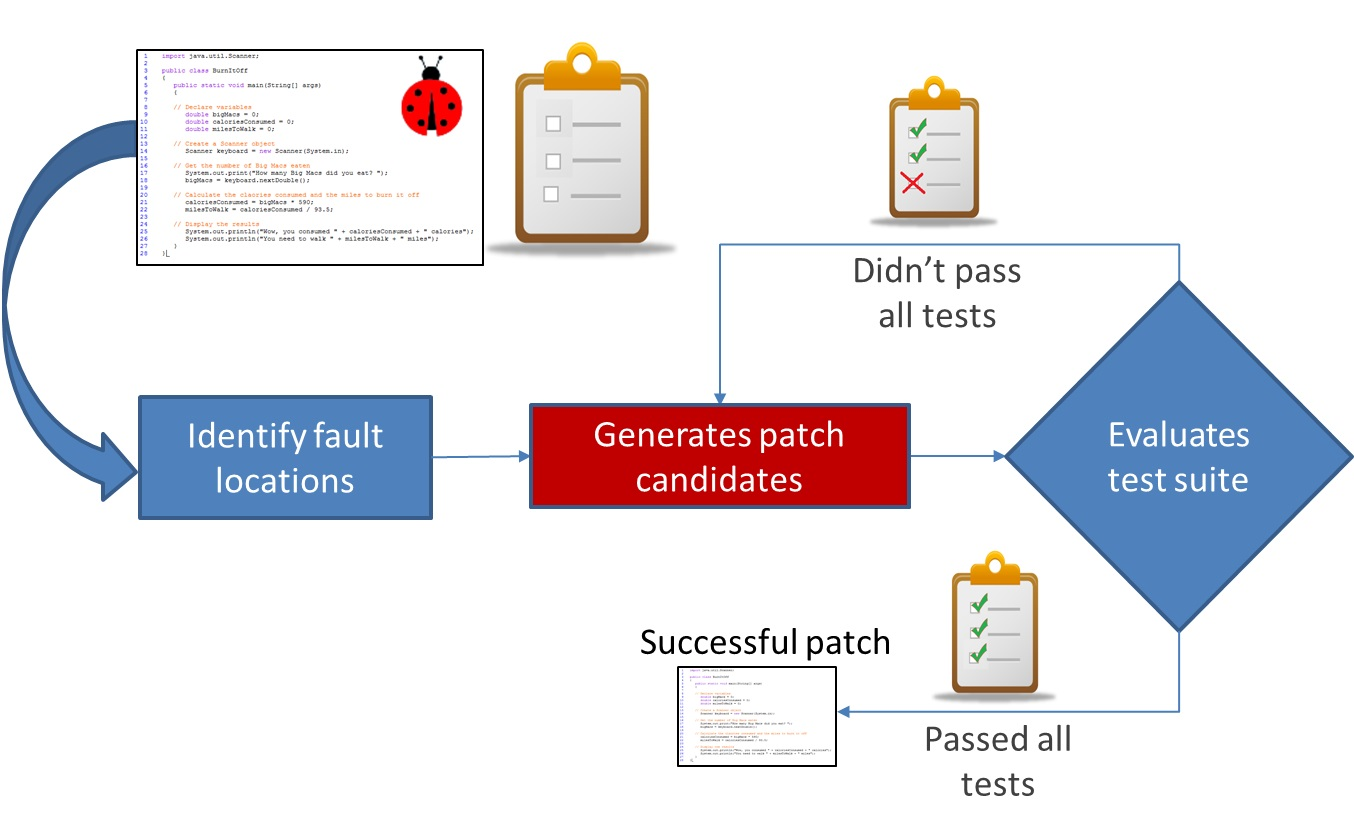
\includegraphics[scale=0.25]{Picture1}
  \caption{Generate and validate approach}
  \label{fig:generateandvalidate}
\end{figure}

The first step of this process is to localize the error to a particular 
statement. There is an extensive list of possible approaches in literature in 
order to perform this tasks~\cite{Jones05,Jones02,Chen02,legoues12,Qi13}, also there are several papers that have focused on the evaluation of the test suite;~\cite{QiICSM13,fan15} the main focus of this paper will be the step between these two, as highlighted in figure~\ref{fig:generateandvalidate} our main focus will be Generating patch candidates.

Once we know where the fault is located we proceed to create what we call 
``Candidate patches". Candidate patches are variations of the original program 
which may or may not be a patch for the bug(s) we are trying to fix. In order to 
create candidate patches we need to apply one or several mutation operators to 
the fault location. 

There are several possible mutation operators that can be applied to a location 
in order to modify the behavior of a program. In order to analyze this we have 
taken mutation operators from two of the most successful approaches in program 
repair that use generate and validate methodology: Genprog~\cite{legoues12} is a very well known and widely used tool that modifies 
statements in order to create candidate patches. PAR~\cite{kim2013} is a 
successful approach that bases their patch generation technique in creating a 
list of commonly used templates of the most used changes that human programmers 
perform in order to fix bugs in their source code. We have denominated these two 
techniques: \textit{Statement-Edition} mutations 
and \textit{Template-Based} mutations.



\subsection{Statement-Edition mutations}
There is a family of well-known approaches such as GenProg~\cite{legoues12} and 
TrpAutoRepair\cite{QiYuhua13} which the main technique for creating candidate 
patches is by applying low level mutation operators (such as append, delete, or 
replace) which modify statements of source code in order to 
repair programs. A statement is the smallest standalone element that expresses 
some action to be carried out in a programming language. This tool is able to 
delete, append or replace statements in order to create candidate patches.

Once the tool has a set of candidate patches, it will run the test suite on each 
of those candidate patches. If it is able to find a candidate patch that can 
pass all the test cases in the test suite, that candidate patch will be 
considered a patch of the bug. If it is not able to pass all the test cases in 
the test suite, then it will go back to creating more candidate patches and will 
continue to do so until it reaches a stopping point, which may be a certain user 
defined number of generations or a user defined clock time limit.


\subsection{Template-based mutations}
A group of researchers have created the approach which they denominate Pattern-based 
Automatic program Repair(PAR), in which they examined a large number of human 
created patches and have abstracted 10 different templates to be the most 
commonly used changes that human programmers perform in order to fix their code~\cite{kim2013}.
The 10 templates which they considered in their approach are the following:
\begin{enumerate}
 \item Null Checker
 \item Parameter Replacer
 \item Method Replacer
 \item Parameter Adder and Remover
 \item Object Initializer
 \item Range Checker
 \item Collection Size Checker
 \item Class Cast Checker
 \item Expression Changer
 \item Expression Adder and Remover
\end{enumerate}

On top of that, in an effort to provide completeness, we also include 6 extra templates that are mentioned in their website (\url{https://sites.google.com/site/autofixhkust/home/fix-templates}) but aren't mentioned in the paper\cite{kim2013}: 

\begin{enumerate}
\item Caster Mutator
\item Castee Mutator
\item Sequence Exchanger
\item Lower Bound Setter
\item Upper Bound Setter
\item Off-by-one Mutator
\end{enumerate}

Due to this, we consider a total of 16 templates.

Another well knownn approach in this domain is the SPR approach~\cite{fan15}, which is composed by a set of transformation schemas as follows:
\begin{enumerate}
\item Condition Introduction
\item Condition Refinement
\item Conditional Control Flow Introduction
\item Insert Initialization
\item Value Replacement
\item Copy and Replace
\end{enumerate}

These transformation schemas can be seen as a generalization of some of the PAR 
templates, for example, ``Condition Introduction" can be seen as a superset of 
the corresponding templates in the PAR approach: Range Checker, Collection Size 
Checker, Class Cast Checker, and Null Checker. ``Condition Refinement" can be 
seen as a superset of 
Expression Adder and Remover. ``Insert Initialization" can be 
generalized from Object Initializer, Upper Bound Setter and Lower Bound Setter; ``Conditional Control Flow Introduction" can be 
seen as a subset of Sequence Exchanger;
``Value Replacement" can be seen as a superset of Method 
Replacer, Parameter Replacer, Castee Mutator and Expression Changer; and ``Copy 
and Replace" can be matched to Expression Adder.

There is enough similarity between these approaches that they can be grouped 
into one category. We have chosen the PAR templates to represent this category 
since these templates provide a more concrete description of how the code is 
being changed, in order for us to replicate it; also, all the SPR templates are represented by one or several of the PAR templates, but not viceversa; and also since the PAR templates 
are written for the Java language, which is a common ground for the rest of the 
approaches considered and the benchmarks to evaluate the approach on.



\section{Building the model}
The first model we built was created based on the 200 Java projects in Github 
with the most stars. When users star a project they are creating a bookmark for 
easier access, and showing appreciation to the repository maintainer for their 
work. Projects with more stars are more popular among the developers of Github 
and therefore more likely to be reviewed by other developers and have higher 
standards of code quality than projects with less stars.

Once we have checked out the 200 Java projects with the most stars, we checkout 
the last 100 bug fixing commits per each project. 

In order to tell apart a bug fixing commit from a non bug fixing commit we 
filter them by applying a regular expression to the commit message:
\\
\\
$[Ff]ix(ed|es|ing)?(\backslash s)*([Bb]ug|[Ii]ssue|[Pp]roblem)?(s)?$
\\
\\
The intuition behind this regular expression is to filter commits where their 
commit message includes phrases such as: ``Fixed issue with variable x", ``Fix for 
problem discussed in meeting", ``Fixing file bug", etc.

We also added two extra filters to our search: First we had commits that only 
modify java source code. This is with the intention of looking only into human 
fixing commits that fix java source code. Developers may also fix bugs in other 
sections of their projects, for example they may fix bugs in bash files, or xml 
code or any other kind of bug, and this wouldn't be relevant to our purpose of 
building a model that looks into the ways in which human developers fix their 
java code.

The last filter we applied to our search is to look only for the fixing commits 
that modify a maximum of 3 files per commit. This is for two reasons: first, we 
want to filter out big merges of code such as pull requests or initial commits 
where the commit is doing much more than just fixing a bug, which are the cases 
that we are interested in; and second, because these approaches usually work 
better when the fault is localized in a small number of locations.

For each of these bug fixing commits, we then checked the version of the code 
before the fix was performed and after the fix was performed. We refer to these 
versions as the ``before-fix" version and the ``after-fix" version.

We then need to know what changes are happening from the before-fix version to 
the after-fix version, and we need to be able to analyze how often these changes 
performed match the mutation operators we are analyzing in order to see what are 
the probabilities of each of them to happen.

In order to do this we used two different widely used tools for mapping changes 
between two versions of code: Gumtree~\cite{falleri14} and QACrashFix~\cite{gao15}.

\todo{Mention some of the heuristics of how we count the instances of the par templates}

These tools create an AST representation of the program files for both the 
before-fix and after-fix representations of the programs for each of the files 
of the commit, and then use a set of heuristics to match the before-fix version 
with the after-fix version. Once this is done, the program's output is a set of 
changes needed to be performed to get from version before-fix to version 
after-fix.

We created two levels in the probabilistic model, the first one we will call the 
\textit{Mutation operator probabilistic model}, and the second level we will 
call the \textit{Replacements probabilistic model}.

The \textit{Mutation operator probabilistic model} is a probabilistic model that 
describes the probabilities to choose between the several different mutation 
operators in a particular fault location.

The \textit{Replacements probabilistic model} is the next level of the 
probabilistic model, which describes, if the ``Replacement" mutation operator is 
picked, what are the probabilities of replacing one statement for another. We 
will explain this in detail below.


\begin{figure}[!h]
  \centering
    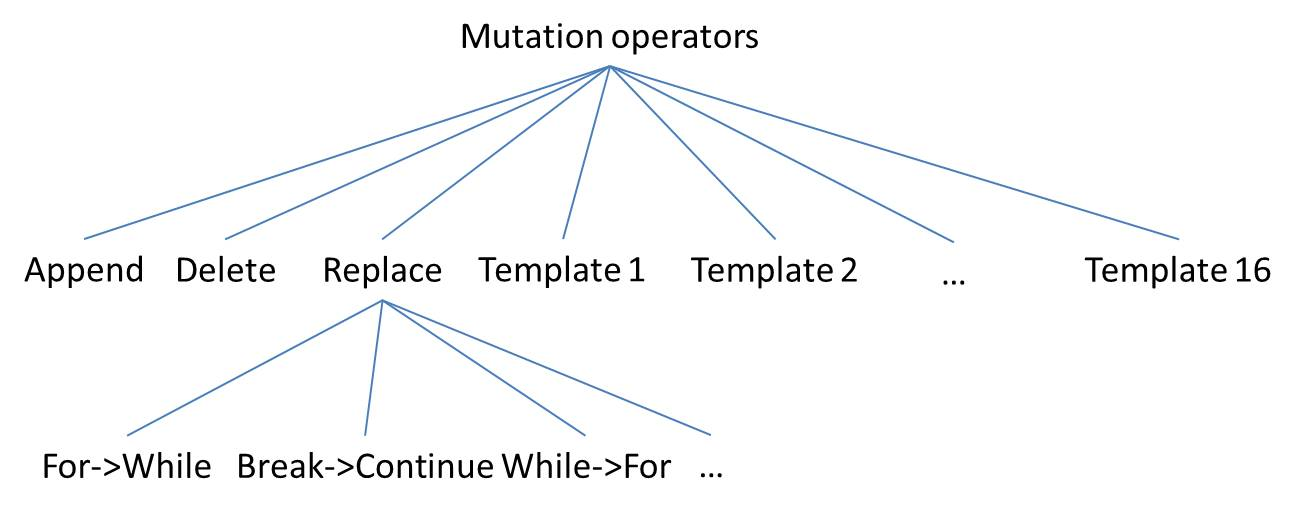
\includegraphics[scale=0.4]{Picture2}
  \caption{Two level probabilistic model}
  \label{fig:probModel}
\end{figure}

\subsection{Mutation operator probabilistic model}
In order to build the \textit{Mutation operator probabilistic model} we created 
a program that goes through these 
changes and matches these changes with the mutation operators we described 
earlier.

We sum the instances of each of the appearances of the mutation operators in the 
lists of changes created out of the differences between the before-fix and 
after-fix versions of each of the files in the 100 last bug fixing commits per 
each of the 200 projects; and these instance sums are the data we take to create 
our probabilistic model.
  


\subsection{Replacements probabilistic model}
In order to build the \textit{Replacements probabilistic model} we created a 
program similar to the one mentioned before (available at https://goo.gl/mMFbnQ
%REPLACE FOR CAMERA READY: https://github.com/mausotog/ReplacementsEmpiricalStudy
Note to reviewer: This link has been aliased for the purposes of the double 
blind review, the content is available, but the reviewer should notice that 
following the link mentioned before will potentially show the identity of the authors) that 
goes through these 
changes and when it encounters a  replacement mutation operator, then it looks 
at what kind of statement is being 
replaced and what kind of statement is replacing the other. We call these 
statements ``replacee" and ``replacer" accordingly.


We analyzed 22 different kinds of statement and the probability in which each of 
them replaces another. For example, what is the probability that a For loop 
would replace a While loop, or the probability that a Break statement would 
replace a Continue statement, etc.

Since there are 22 statement types that we analyzed and each of these 22 may 
replace each of these 22 statement types, we then have 484 combinations of 
replacement combinations. 

It is also worth noticing that these probabilities are not reciprocal, meaning 
that the probability of a For loop replacing a While loop is different from the 
probability of a While loop replacing a For loop, and the same applies to all 
the different statement types.


\section{Sanity Check}
The first step in our effort to check if the probabilistic model is going in the 
right direction is to perform a sanity check on the model.

We performed two different sanity checks, the first of which is a 10 fold cross 
validation of the model; and second, a run on an initial example to check how 
much faster we can find a patch with the probabilistic model vs the equally 
distributed approach. Following, we will describe these two steps:

\subsection{10 fold cross validation}

Our initial sanity check was performed on the replacements model. At this point, 
our initial probabilistic model, built from 200 projects was segregated into 10 
different folds, each fold had 20 projects assigned at random. For each of the 
folds we would take 1 fold for testing and the remaining 9 folds for training. 
Afterwards we analyze how often do the training data is able to predict the 
testing data. These is performed 10 times, one time per each fold and then it is 
averaged to see how commonly is the training data able to predict the testing 
data.

In this initial sanity check we are comparing two distributions: the sub-model 
that is built from the remaining 9 folds, and the distribution of the testing 
data. We need to analyze how often one of the distributions (the sub-model 
training data) predicts the other distribution (the distribution of the fold we 
are trying to predict). 

Since the main focus of this step is to check whether the behavior of the 
current approaches would perform faster with the probabilistic model as opposed 
to the current equally distributed scheme; we rank the first five choices each 
of the models would take and see how many of the instances in the testing data 
match those first five guesses.

\begin{figure}[!h]
  \centering
    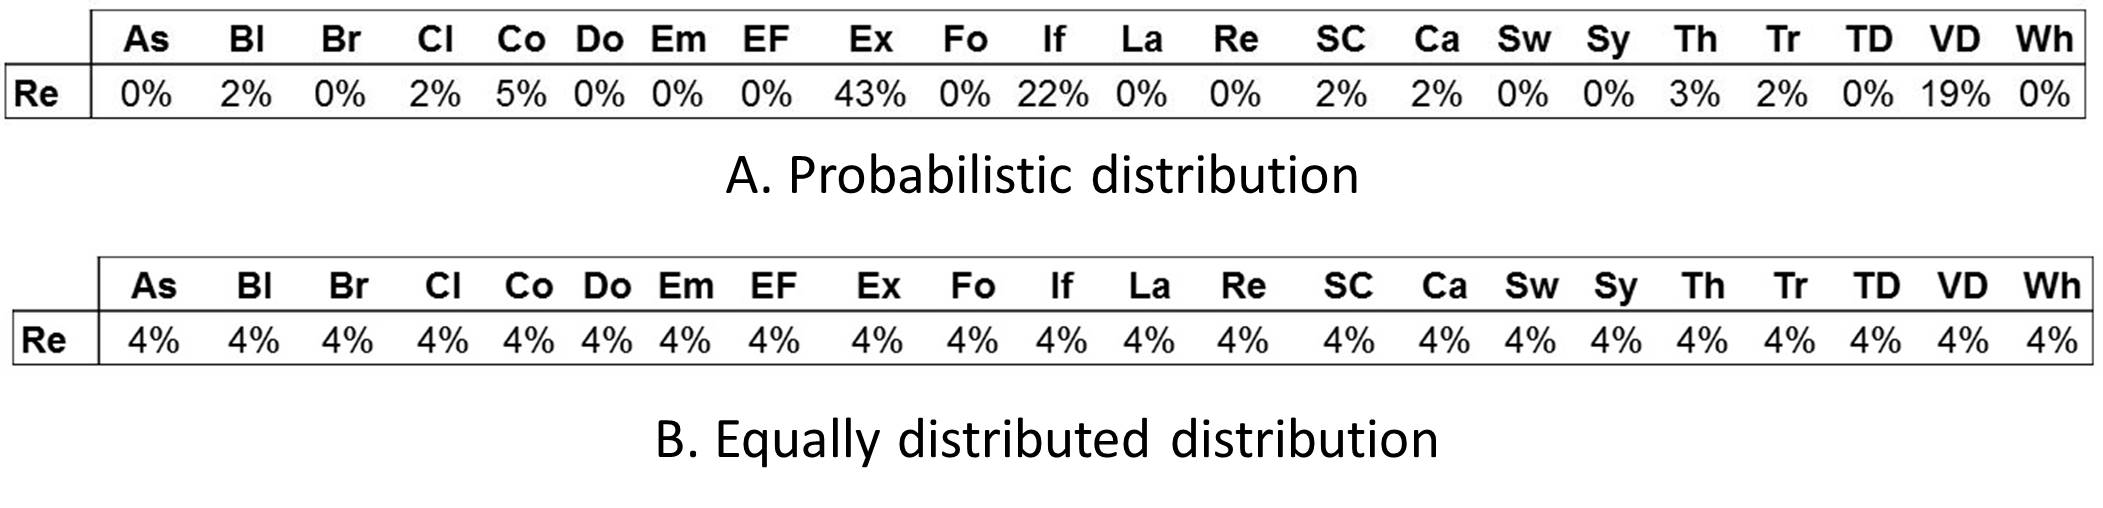
\includegraphics[scale=0.25]{sanity5}
  \caption{A) Example of the Return Statement row of a sub-model created from 
the 
training data. B) Example of Return Statement with Equally Distributed 
probability}
  \label{fig:exPredReturn}
\end{figure}

To illustrate the point, let's take a simple example. Assume we have a 
distribution in fold 1 that describes how many times each statement is replaced 
by other kinds of statements in this fold 
only, this is what we denominate testing data and we represent it with $E_{n,m}$ 
where $n$ is the statement being replaced (replacee) and $m$ the statement it is 
replaced by (replacer); likewise we have a probabilistic sub-model created from 
folds 2-10 inclusive $TP_{n,m}$ where $\forall n,m: 1<=n<=22 \land 1<=m<=22$, 
that describes how often each statement is replaced by 
other kinds of statements, this is what we call the training data. 

In 
particular, assume we are analyzing the Return statement (Row 13). We want to 
predict 
how well the sub-model created from folds 2-10 is able to predict the testing 
data; in this particular case, how well is the section of the sub-model that 
describes the Return Statement able to predict the instance count of the 
statements that replace a Return Statement in the testing data.

Assume the training data is a sub-model $TP_{n,m}$ which contains a row 
$TP_{13,m}$ as the one shown in Figure 
\ref{fig:exPredReturn}A, and the testing data is a distribution that describes 
how many instances of returns were replaced by different statements as follows: 
A return statement was replaced by a Expression Statement 4 times $E_{13,9} = 
4$; by an If 
Statement 2 times $E_{13,11} = 2$; by a Continue Statement 2 times $E_{13,5} = 
2$; by a Do Statement 1 time $E_{13,6} = 1$;
and by a Try Statement 1 time $E_{13,19} = 1$. As a clarification, this is a 
fictional example 
to explain how the prediction is being analyzed.

For each of the statements we would take the top five guesses from each row in 
the sub-model and see how many instances of the testing data were correctly 
predicted. In this example, the top five guesses in this row would be: The most 
likely statement chosen to replace a Return Statement according to this row in 
this fictional sub-model would be a Expression Statement (Ex) $TP_{13,9} = 43\%$ 
which means that there is a 43\% of probability to replace a Return Statement. 
The second most likely would be an If Statement (If) $TP_{13,11} = 22\%$ this 
means there is a 22\% chance to get chosen to replace a Return statement. 
Following, the next most likely statements chosen by the 
sub-model would be  Variable Declaration (VD)  $TP_{13,21} = 19\%$, next is 
Continue Statement (Co)  $TP_{13,5} = 5\%$, and last of the five top guesses 
would 
be Throw Statement (Th) $TP_{13,18} = 3\%$.

We then compare how many instances of the testing data were correctly predicted 
by these top five guesses of this row in the sub-model. In this example, we will 
look at the instances that match the top five guesses in the testing data, which 
would be: Expression Statement $E_{13,9} = 4$, If Statement $E_{13,11} = 2$, and 
Continue Statement $E_{13,5} = 2$. Since Do 
Statement $E_{13,6} = 1$ and Try Statement $E_{13,19} = 1$ were not within the 
top five guesses, then the 
instances in these two categories won't be considered a successful match, but 
the former three would. 

Based on this information, we can say that the 4 instances of Expression 
Statement replacing a Return Statement in the testing data were correctly 
predicted by the sub-model; the same with the 2 instances of the If Statement 
and the 2 instances of the Continue Statement. The instance of the Do Statement, 
and the instance of the Try Statement, would be considered as not correctly 
predicted by the sub-model. In this case, since the sub-model correctly 
predicted 8 out of 10 instances, we say that the sub-model correctly predicted 
80\% of the instances in the testing data. 

In order to contrast this with the equally distributed approach used currently, 
we assign all the statements, the same probability of being chosen to replace 
the statement being analyzed. We denominate the equally distributed approach 
$TE_{n,m}$ where $\forall n,m: 1<=n<=22 \land 1<=m<=22 \land TE_{n,m} = 4.54\%$. 
We have been analyzing the Return Statement in this particular example, as 
detailed in Figure \ref{fig:exPredReturn}B. To get the top five choices of the 
equally distributed schema we just pick five choices at random, since all of 
them have the same probability, which is how the current approach handles what 
statement to pick.

For example, if the approach picks at random the statements: Assert Statement 
$TE_{13,1}$, 
Do Statement $TE_{13,6}$, Expression Statement $TE_{13,9}$, Throw Statement 
$TE_{13,18}$ and Try Statement $TE_{13,19}$. Then we 
would match how many of the instances in the testing data were correctly 
predicted by this equally distributed schema.

In this example, the 4 instances of Expression Statement $E_{13,9} = 4$, the 
instance of Do 
Statement  $E_{13,6} = 1$, and the instance of Try Statement $E_{13,19} = 1$ 
would be considered to be correctly 
predicted; while the 2 instances of If Statement $E_{13,11} = 2$, and the 2 
instances of 
Continue Statement $E_{13,5} = 2$ would be considered to be incorrectly 
predicted. Since the 
equally distributed approach in this example correctly guessed 6 out of 10 
instances of the testing data, we would then say that in this particular case, 
the equally distributed approach correctly predicted 60\% of the instances in 
the testing set.  

We ran this experiment with all the rows $n$ in the sub-model $TE_{n,m}$ and 
$TP_{n,m}$ for each of the 10 
folds. The results are detailed in Figure \ref{fig:results10fcv}. As we can see 
in this graph, the red bars represent the results of the percentage of correctly 
predicted instances of the testing data in each particular fold; while the blue 
bars represent the percentage of correctly predicted instances using the top 5 
guesses of the sub-model of each of the folds. We have a mean of 19.79\% 
correctly predicted instances through the different folds when using the equally 
distributed schema, while we get a mean of 87.70\% correctly predicted instances 
through the different folds when using the probabilistic model. 



\begin{figure}[!h]
  \centering
    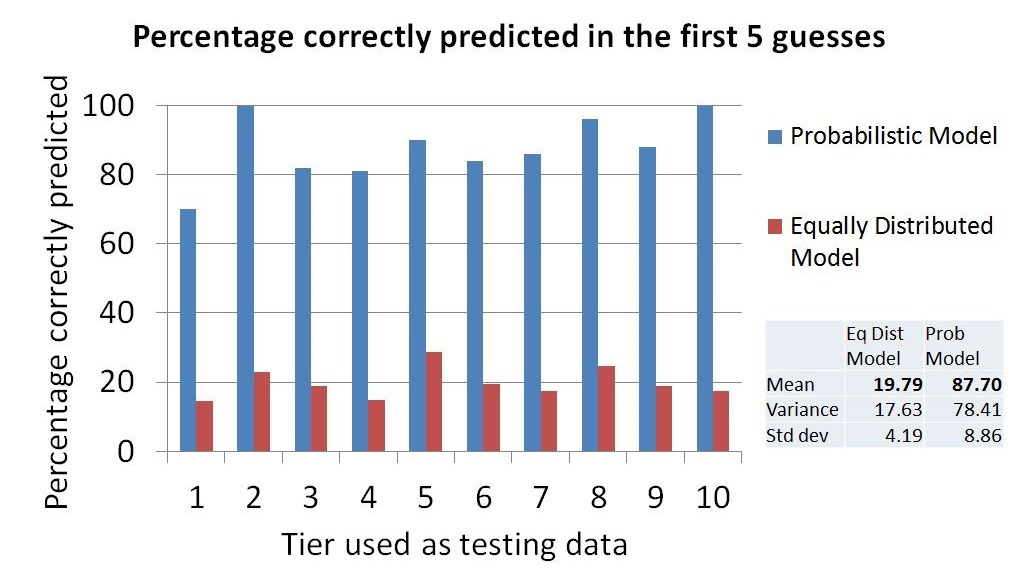
\includegraphics[scale=0.33]{sanity1}
  \caption{Results 10 fold cross validation}
  \label{fig:results10fcv}
\end{figure}

\subsection{Initial Example}
After performing the 10 fold cross validation, we know that the model built from 
gathering cases from mined from Github predicts with very high accuracy all the 
subsets of the data gathered, which implies that the data is consistent among 
the folds and outperforms the current equally distributed model in every case. 

The natural next step would be to try the model with an example taken from 
outside of the collected cases from Github. Therefore we evaluated our model 
with an example of a basic bug in a method as shown in figure 
\ref{fig:initialExample}. The purpose of this method is to calculate the median 
of three numbers, and there is a bug as indicated by the highlighted text where 
instead of $ret = z;$ it should be $ret = x;$ in order to have a correct output 
for all cases.

\begin{figure}[!h]
  \centering
    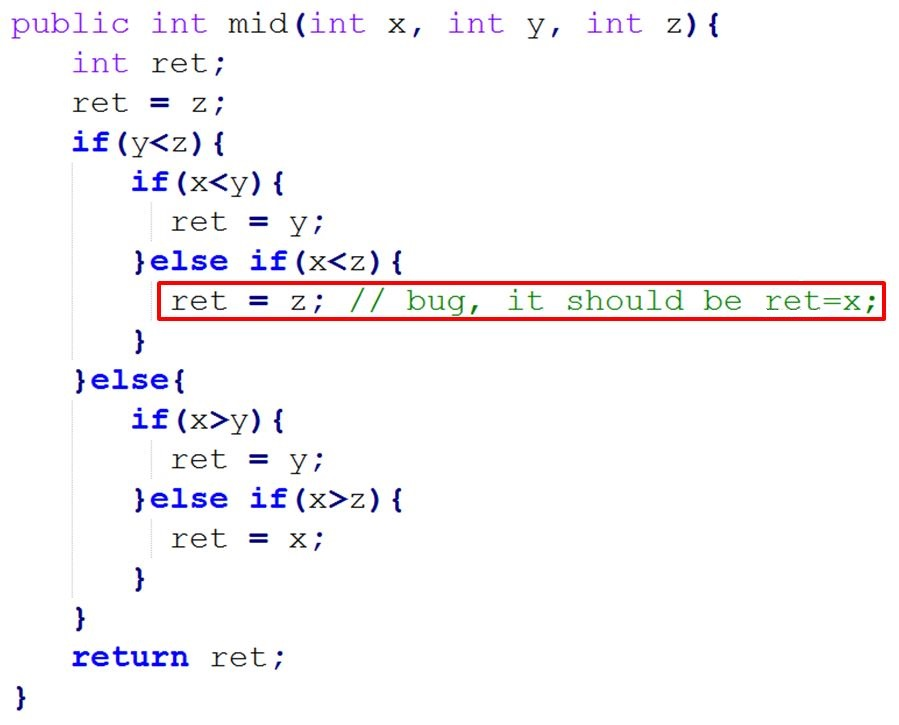
\includegraphics[scale=0.35]{sanity2}
  \caption{Initial example}
  \label{fig:initialExample}
\end{figure}

In order to be able to do this, we restructured the code of the tool ``GenProg4J" 
\todo{or GenProg4Java, I don't know what Claire prefers} (available at 
https://bitbucket.org/clegoues/genprog4java/), which is the Java version of the 
well known tool Genprog~\cite{legoues12}. This tool provides all the work-flow 
for any generate-and-validate approach to be implemented. We restructured the 
tool in order to be able to select the mutation operators between a 
probabilistic model, and the default (equally distributed).

We then ran the tool with the code in figure \ref{fig:initialExample} using both 
the probabilistic model and the equally distributed model. Since this is an 
initial example for sanity checking, we start by evaluating it on a subset of 
the mutation operators. We first evaluate it with$ Replace only$ and $Append, 
Remove and Replace$. The results are detailed in figures 
\ref{fig:resultsReplace} and \ref{fig:resultsARR}. 

Generate-and-validate, as explained before, works by creating variants of the 
source code by applying mutation operators to the original source code. 
Therefore, a large number of variants created before finding a patch means that 
it takes longer to find a patch, than a small number of variants. Which means 
that in these graphs, the smaller number of variants in each case, means that 
the patch was found faster, than with a larger number of variants. It is also 
noticeable that this tool uses genetic programming in its workflow, therefore we 
run the tool with 10 different seeds in order to be able to abstract the results 
and not focus on a particular seed.

In figure \ref{fig:resultsReplace} we consider only the mutation operator 
$Replace$, which means, that the tool will disregard all other mutation 
operators and will only apply Replace operations using the probabilistic model 
of Replacements. This is because at this step we are evaluating our model in a 
subset of the mutation operators to see if it makes sense to move forward and 
continue implementing the rest of the mutation operators.

In this graph we can see the runs with 10 different seeds, contrasting the 
number of variants it takes to find a patch using the probabilistic approach 
(blue bar), with the number of variants it takes to find a patch using the 
equally distributed approach (green bar). 

As we can derive from the graph, the probabilistic approach was able to find a 
patch faster than the equally distributed for all the seeds tested. In some 
cases as seed 5, 7 and 10, the patch using the probabilistic approach was found 
in one of the first variants, therefore the number is so low that it doesn't 
show in the graph. In average, we found that using the probabilistic model we 
could find a patch in 23.8 variants, while it took an average of 60.5 variants 
to find a patch using the equally distributed model.

\begin{figure}[!h]
  \centering
    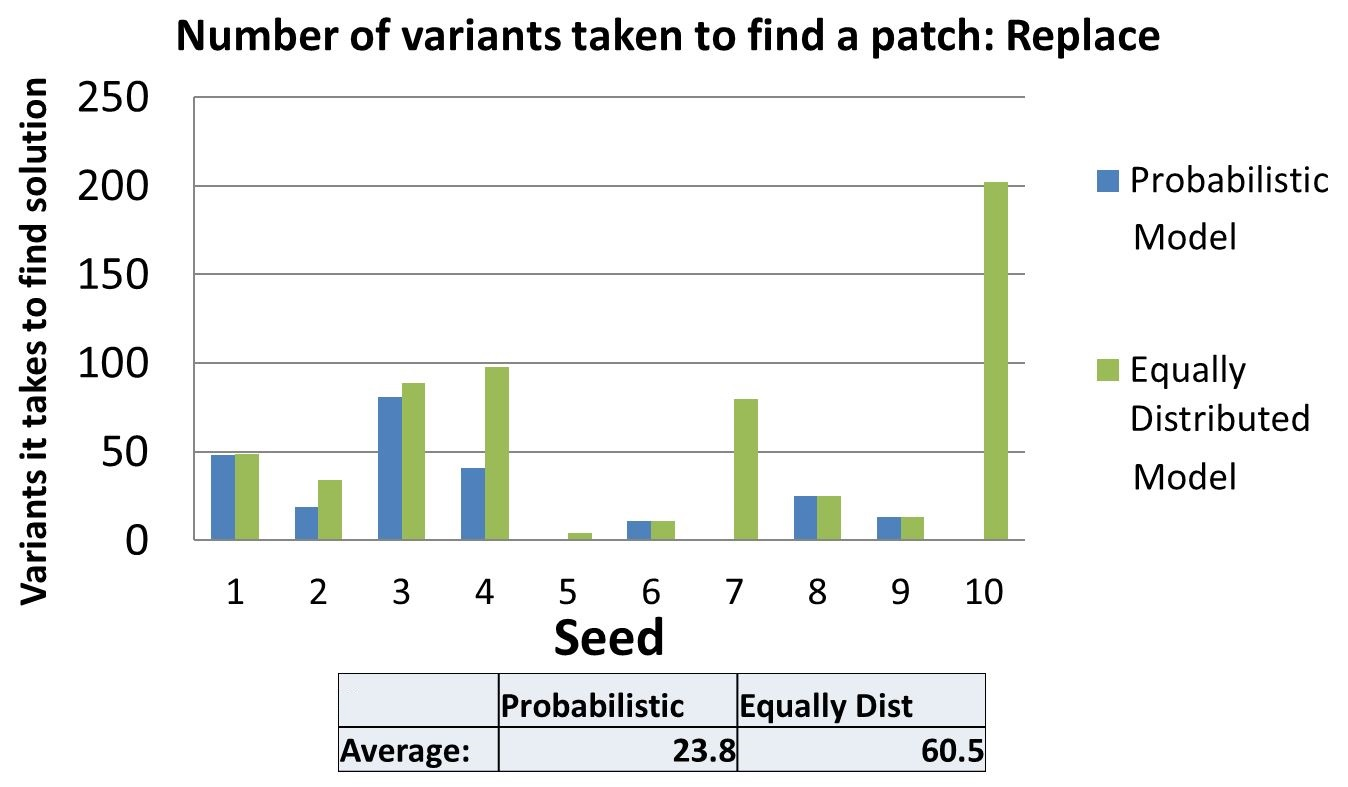
\includegraphics[scale=0.25]{sanity3}
  \caption{Using replace to guide the search for a patch of the initial example}
  \label{fig:resultsReplace}
\end{figure}

In figure \ref{fig:resultsARR}, we consider three mutation operators: Append, 
Remove and Replace. In this case we can also notice that in seeds 7 and 10 the 
number of variants it takes to find a patch using the probabilistic model is 
close to 1 therefore it is hard to notice it in the graph. In this case the data 
shows that using the probabilistic model model we get a mean of 22.6 variants 
before finding the patch, while it takes an average of 41.4 variants to find the 
patch using the equally distributed approach.

\begin{figure}[!h]
  \centering
    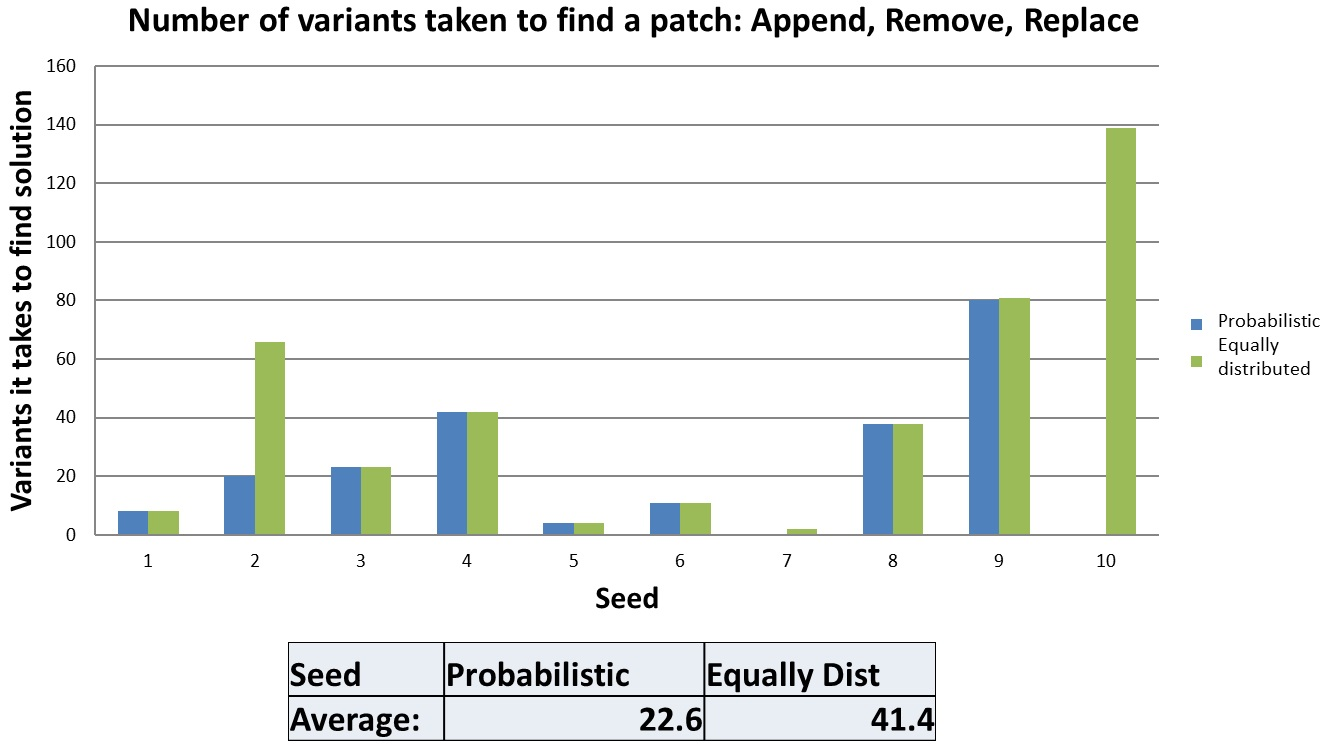
\includegraphics[scale=0.25]{sanity4}
  \caption{Using append, remove and replace to guide the search for a patch of 
the initial example}
  \label{fig:resultsARR}
\end{figure}

\section{Upgrading the model}
After having very successful results in the sanity checking process, we decided 
to improve our model by building it from the 500 projects in Github with more 
stars. This is the model generated from the largest code base so far to the best 
of our knowledge, surpassing all the previous state of the 
art~\cite{long15,Soto15,zhong15,matias15}. At this point, in our analyzed data, 
we found that the Template-Based mutations comprise 29.26\% of the corpus of 
instances found, while Statement-Edition mutations make up 70.74\% of the 
corpus.

Since this idea seems promising at this point we decided to implement the rest 
of the mutatio
n operators. There are several different template-based approaches 
\cite{kim2013,fan15,long15} which are constituted by mining common behaviors 
that developers usually perform to patch errors in their code. Since these 
templates in the different approaches tend to be very similar, we considered the 
approach that seems to be representative of the template-based category due to 
the diversity of the templates it encounters. 

``Automatic patch generation learned from human-written patches"~\cite{kim2013} describes 10 different templates that 
developers use very commonly to patch their code. Besides these 10 templates 
published, they define other extra 6 templates in the research site 
https://sites.google.com/site/autofixhkust/home/fix-templates that we have 
considered as a representation of the template-based mutation operators.

We implemented these 16 templates in GenProg4J, and generated the functionality 
to be able to select which subset of mutation operators to apply in a particular 
run.

\section{Evaluation}
We are interested in evaluating our new approach with real life bugs taken from 
open source projects that have a long history of maintainability and 
scalability. For these reasons, we chose Defects4j~\cite{just14} as our 
evaluation platform. Defects4j~\cite{just14} is ``a database and extensible 
framework providing real bugs to enable reproducible studies in software testing 
research"~\cite{just14}. This database bugs contains 357 real bugs from 5 
real-world open source programs, and each of these cases is accompanied by a 
comprehensive test suite that can expose the bug. This database also provides 
the corresponding human-generated patch, which is the edits performed by a human 
developer to patch the bug.

For this evaluation we tested the mutation operators using three different sets 
of operations: 1) Statement-Edition mutations only 2) Template-based mutations 
only 3) All mutations.


\subsection{Single line bugs with Human Injected Fault Localization}
Since historically automatic program repair has worked better with single line 
patches, we decided to first test bugs that required a single line edit to get 
patched. We analyzed the first 3 bugs from each of the projects that required a 
single line edit. Therefore we analyze the bugs that met this criteria: Chart 1, 
Chart 8, Chart 20, Closure 10, Closure 14, Closure 18, Lang 6, Lang 16, Lang 21, 
Math 2, Math 5, Math 10, Time 4, Time 16 and Time 19.

From these 15 bugs we were able to find patches for 5 of them as described in table \ref{tab:singleLineBugs}. It is also worth mentioning that the numbers shown in the table are the mean from the solutions found running the tool with 20 different seeds. 

In the first row (Closure \#10) we can see that in all three comparisons (Statement-Edition Only, Template-Based Only, and All mutations), the approach using the Probabilistic model performs better than its counterpart using the equally distributed model. This happens as well in all cases of bugs Math \#2 and Time \#19 except for the cases where no patch was found. Different from this, in bugs Chart \#1 and Closure \#18 the equally distributed approach finds a patch faster in average. This is due to the fact that removal mutations such as Deletion and Expression Changer are more likely to be picked by the equally distributed model than the probabilistic model since developers use these editions less often than others. But these editions have been seen in the past to make the test cases pass even if the edition did not fixed the bug as per the opinion of developers as indicated in~\cite{kim2013}.

\begin{table*}
	\centering
	\resizebox{\textwidth}{!}{
\begin{tabular}{|r||rr|rr|rr|}
\hline 
  &\multicolumn{2}{c|}{\textbf{Stmt-Edition}} & \multicolumn{2}{c|}{\textbf{Temp-Based}} & \multicolumn{2}{c|}{\textbf{All mutations}} \\  
 \hline
 \textbf{Bug Name}  & \textbf{Equally Dist} & \textbf{Probabilistic} & \textbf{Equally Dist} & \textbf{Probabilistic} & \textbf{Equally Dist} & 
\textbf{Probabilistic} \\
 \hline 
 Closure \#10 & 221.0 & 179.5 & 183.1 & 121.3 & 163.3 & 157.4 \\
 \hline
 Closure \#18 & Not found & Not found & 36.2 & 197.5 & 45.0 & 139.0 \\
 \hline
 Math \#2 & Not found & Not found & 109.4 & 39.6 & 109.4 & 39.6 \\
 \hline
 Time \#19 & 94.1 & 80.7 & Not found & Not found & 135.1 & 91.9 \\
 \hline
 Chart \#1 & 1.8 & 7.3 & 4.9 & 19.0 & 2.2 & 4.8 \\
 \hline 
\end{tabular}
}
		\caption{Single line bugs With Fault Injected Fault Localization}\label{tab:singleLineBugs}
\end{table*}



\subsection{Bugs fixed with a single line edit}
Last evaluation with the bugs we found had a fix


\subsection{Bugs fixed with a multi line edit within a function}
Last evaluation with the bugs we found had a fix

\section{Discussion}
Section text here.





\section{Conclusion}
The conclusion goes here.




% conference papers do not normally have an appendix


% use section* for acknowledgment
\section*{Acknowledgment}
The authors would like to thank...





% trigger a \newpage just before the given reference
% number - used to balance the columns on the last page
% adjust value as needed - may need to be readjusted if
% the document is modified later
%\IEEEtriggeratref{8}
% The "triggered" command can be changed if desired:
%\IEEEtriggercmd{\enlargethispage{-5in}}

% references section

% can use a bibliography generated by BibTeX as a .bbl file
% BibTeX documentation can be easily obtained at:
% http://mirror.ctan.org/biblio/bibtex/contrib/doc/
% The IEEEtran BibTeX style support page is at:
% http://www.michaelshell.org/tex/ieeetran/bibtex/
%\bibliographystyle{IEEEtran}
% argument is your BibTeX string definitions and bibliography database(s)
%\bibliography{IEEEabrv,../bib/paper}
%
% <OR> manually copy in the resultant .bbl file
% set second argument of \begin to the number of references
% (used to reserve space for the reference number labels box)
%\begin{thebibliography}{1}

%\bibitem{IEEEhowto:kopka}

%\end{thebibliography}

\bibliographystyle{abbrv}
\bibliography{sigproc}  % sigproc.bib is the name of the Bibliography in this case
% You must have a proper ".bib" file
%  and remember to run:
% latex bibtex latex latex
% to resolve all references



% that's all folks
\end{document}


